\documentclass[a4paper, 10pt]{ctexart} %中文支持
\usepackage{float}              %防止浮动元素浮动
\usepackage{rotating}           %旋转图片
\usepackage{hyperref}           %生成可跳转的书签
\usepackage{amsfonts}           %对某一些字体之支持
\usepackage{amsmath}          %数学公式
\usepackage{amsthm}             %定义, 定理, 证明, 例子环境的支持
%使用方法:
%\newtheorem{environment name}{caption}
%比如 \newtheorem{example}{这是例子}
%效果 \begin{example} xxx \end{example} -> 这是例子 1 xxx
%proof就不需要了
\usepackage{graphicx}           %插入图片
\usepackage[left=1.5in,right=1.5in,top=1in,bottom=1in]{geometry}   %用来排版的
\usepackage[]{color}            %给部分文本上色的
\usepackage{algorithm}          %写伪代码的
\usepackage{algorithmic}        %同上
\usepackage{minted}             %书写代码
\usepackage{amssymb}            %用来加入一些数学符号, 比如说 $\varnothing$
\usepackage{fontspec}           %不知道用来干嘛的
\usepackage{titlesec}           %用来调整section等的大小和字体
\pagestyle{plain}
\titleformat*{\section}{\huge\bfseries}
\titleformat*{\subsection}{\Large\bfseries}
\titleformat*{\subsubsection}{\large\bfseries}
% 日, content里的不还是没变? 难堪的一笔

\setmonofont{Ubuntu Mono}       %?
\usemintedstyle{custommanni}    %设置minted插入代码的风格

\newtheorem{theorem}{定理}
\newtheorem{example}{Example}
\newtheorem{definition}{定义}
\newtheorem{lemma}{引理}
\newtheorem{proposition}{命题}
\title{single-source shortest paths}
\begin{document}
\begin{titlepage}
    \maketitle
\end{titlepage}
\tableofcontents


\section{intro and prequisition}
\subsection{Notation}

我们研究最短路径的话, 我们必然会面对图的各种参数, 因为我们当然是在有权图上面寻找最短路径的, 如果说是那种将路径长度定义为路径所经过的节点个数的话, 正如22所讲的那样的话, 
这种就不在我们这次的研究范围内了. 于是我们给定的是 {\bf 有权, 有向图}. 

\begin{definition}
    A graph is abbreviated as $G  = \left(V, E\right)$ , 这是我们已经熟知的. 
\end{definition}

\begin{definition}
一个path记为 $p$ , 可以写为 $\left< v_{0}, v_{1}, \cdots , v_{n}\right>$ , 为了突出其终点和起点, 一个path可以记为
$$p: u \leadsto v$$
\end{definition}

\begin{definition}
$w : E \to \mathbb{R}, \left(u , v\right) \mapsto w \left(u , v\right)$ , 将权重以函数的方式写出来当然是为了严谨. 
虽然在一些人看来可能是脱裤子放屁, 但其实有很多东西的定义都是这样用函数定义的. 同时也定义了path的权重 $p \mapsto w \left( p\right) = \sum\limits_{i=1} ^{\infty} w \left( v_{i}\right)$
\end{definition}

\begin{definition}
最短路径的记号: 
\[
\delta \left(u , v\right) = 
\begin{cases}
    \min \left\{w \left(p\right) : p: u \leadsto v \right\}, &\text{ if there is a path from u to v} \\
    \infty, & \text{ otherwise}
\end{cases}
\]
\end{definition}


\subsection{some variants of single-source shortest paths}
我们目前的问题称为 single-source shortest paths. 对于有权有向图, 给定了一个source, 我们要找出从source到其他点的最短路径的大小, 以及可以求解出这个路径. 
single-source shortest paths 问题有多种变体, 当然这里只是介绍一下
\begin{figure}[H]
    \centering
    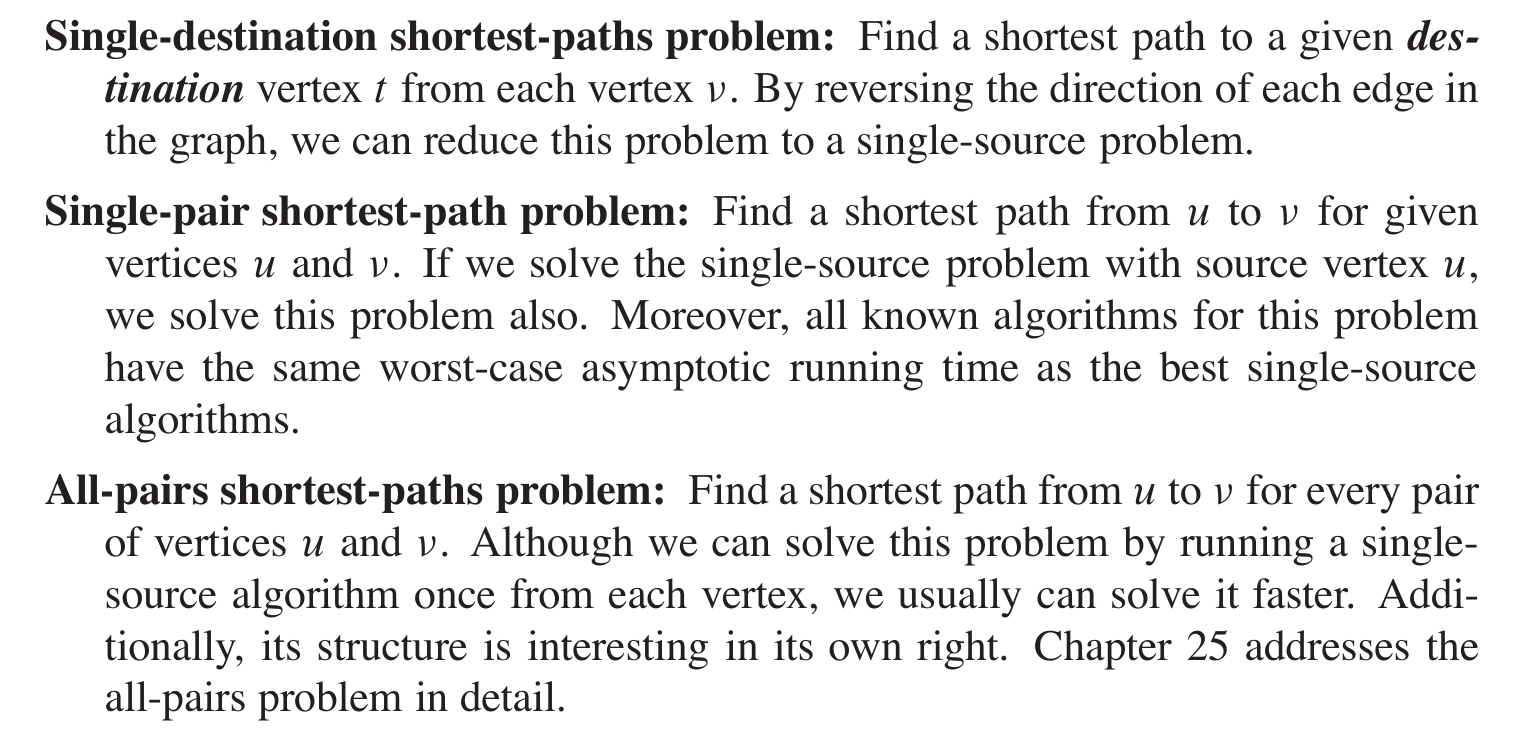
\includegraphics[scale = 0.3]{sssp1.png}
    \caption{the variants of single-source shortest paths problems}
    \label{1}
\end{figure}
其中这里的all-paired shortest paths problems 是我们在25中面对的问题. 

\subsection{optimal structure of shortest paths}
rt. 最短路径具有优化子结构, 即, 
\begin{theorem}
最短路径的{\bf 子路径}也是{\bf 最短路径}
\end{theorem}
\begin{proof}
    trivial!
\end{proof}


\subsection{representation of shortest paths} 
这涉及到前面我还没看的部分, 即无向无权图的最短路径求解. 这里我们涉及 \textbf{predecessor} , 符号 $\pi  $ 的出现说明其和 \textbf{predecessor} 有关. 比如说: 
$v. \pi$ 是 $v$ 的一个前驱
%目前并不清楚这个前驱是哪里来的. 
\begin{definition}[predecessor subgraph]
$G_{\pi} = \left(V_{\pi  } , E_{\pi}\right)$ 是 predecessor subgraph , 其中 
$$V_{\pi} = \left\{v \in V : v.\pi \ne \varnothing\right\}\cup \left\{s\right\}$$ 
s 是source, 
并且
$$E _{\pi   } = \left\{ \left(v.\pi , v\right):v \in V_{\pi} - \left\{s\right\} \right\}$$
\end{definition}

虽然这里定义并不是非常清晰, 比如说 $v.\pi$ tm的是什么我也不太清楚. 但是我们这里可以用语言将其描述清楚:
\\ [8pt]
\noindent single-source shortest paths 问题其实就是求出下面这个子图 
\\$G'  = \left(V '  , E'\right)$ \\ $V'$ 是所有能够达到的点的集合, 即 $\delta \left(s , v\right) \ne \infty$
\\并且 $G'$ 是一个树, 并且这个树上的任意一个节点 $v$ , 则 $v$ 和 $s$ 之间的距离最短. 

这就是用另一种方法说了一边我们要求什么. 
超, 我也不知道为什么要说什么 predecessor subgraph . 可能是说 $G'$ 是 $G_{\pi    }$ 的子图. 并不是很懂
\subsection{relaxation}
\subsubsection{initializing single source}
我们使用 $v.d$ 表示目前已知的 $v, s$ 之间的距离. 称为 \textbf{shortest path estimate}. 这时可以补充上面的 $v.\pi$ 了: $v.\pi$ 就是目前已知的 "最短路径上" $v$ 的前驱.

\begin{figure}[H]
    \centering
    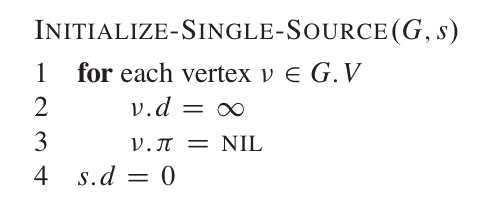
\includegraphics[scale = 0.5]{sssp2.png}
    \caption{初始化的伪代码}
    \label{iss}
\end{figure}




\subsubsection{relaxation: code and definition}

relaxation是一个很简单但是很重要的操作. relaxation这个词我们之前就已经见过了, 可能有人那时候开始就觉得: 
松弛是什么几把叫法啊. 总之, 鬼知道, 确实不够自然. 
应该可以将其称为renew或者update. 

\begin{definition}[relaxation]

\end{definition}
\subsection{some property}

你可以将两点之间的最短路径视为一个度量, 即, $\delta \left(u ,v\right)$ , 至少在正权图中, 满足度量的三个性质: 

\begin{itemize}
    \item 
    1. 正定性: $\delta \left(v, u\right) \ge 0$
    \item 
    2. 忘了什么性: $\delta \left(u,v\right) = 0   \implies u = v$ 
    \item
    3. 三角不等式. $\delta (u, v ) + \delta \left(v , w\right) \ge \delta (u ,w)$
\end{itemize}

至少这样好像挺有意思的. 
\section{Bellman-Ford algorithm}
\subsection{an introd}
\subsection{algorithm}
\subsection{negative weighted cycles}
\subsection{the prf of theorem}
\section{Dijikstra algorithm}
\subsection{an review}
\subsection{algorithm}
\subsection{the prf of algorithm}
\end{document}